
\resizebox{0.25\textwidth}{!}{%
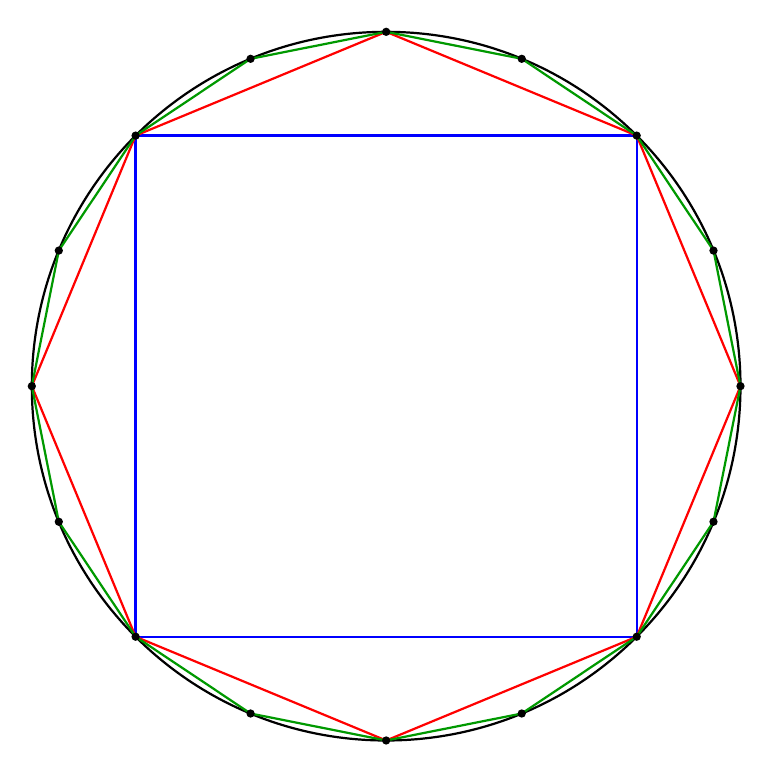
\begin{tikzpicture}[scale=1.5, line width=0.8pt]

% Promien okregu
\def\R{3}

% ---------- Okrag opisany ----------
\draw[black, thick] (0,0) circle (\R);

% ---------- Kwadrat obrocony o 45 stopni ----------
% Wierzcholki kwadratu: katy 45, 135, 225, 315
% Wspolrzedne:
%   45°:  (R*cos45, R*sin45) = (R/sqrt2, R/sqrt2)
%   135°: (-R/sqrt2, R/sqrt2)
%   225°: (-R/sqrt2, -R/sqrt2)
%   315°: (R/sqrt2, -R/sqrt2)
\draw[blue, thick] 
  ({-\R/sqrt(2)},{\R/sqrt(2)}) -- 
  ({\R/sqrt(2)},{\R/sqrt(2)}) -- 
  ({\R/sqrt(2)},{-\R/sqrt(2)}) -- 
  ({-\R/sqrt(2)},{-\R/sqrt(2)}) -- cycle;

% ---------- Foremny osmiokat ----------
% Wierzcholki co 45 stopni: 0, 45, 90, 135, 180, 225, 270, 315
\draw[red, thick] 
  (\R,0) --
  ({\R/sqrt(2)},{\R/sqrt(2)}) --
  (0,\R) --
  ({-\R/sqrt(2)},{\R/sqrt(2)}) --
  (-\R,0) --
  ({-\R/sqrt(2)},{-\R/sqrt(2)}) --
  (0,-\R) --
  ({\R/sqrt(2)},{-\R/sqrt(2)}) -- cycle;

% ---------- Foremny szesnastokat ----------
% Wierzcholki co 22.5 stopni: 0, 22.5, 45, 67.5, 90, ...
\draw[green!60!black, thick] 
  (\R,0) --
  ({cos(22.5)*\R},{sin(22.5)*\R}) --
  ({\R/sqrt(2)},{\R/sqrt(2)}) --
  ({cos(67.5)*\R},{sin(67.5)*\R}) --
  (0,\R) --
  ({cos(112.5)*\R},{sin(112.5)*\R}) --
  ({-\R/sqrt(2)},{\R/sqrt(2)}) --
  ({cos(157.5)*\R},{sin(157.5)*\R}) --
  (-\R,0) --
  ({cos(202.5)*\R},{sin(202.5)*\R}) --
  ({-\R/sqrt(2)},{-\R/sqrt(2)}) --
  ({cos(247.5)*\R},{sin(247.5)*\R}) --
  (0,-\R) --
  ({cos(292.5)*\R},{sin(292.5)*\R}) --
  ({\R/sqrt(2)},{-\R/sqrt(2)}) --
  ({cos(337.5)*\R},{sin(337.5)*\R}) -- cycle;

% ---------- Wierzcholki (kropki) ----------
% Wspolne wierzcholki: co 45 stopni (kwadrat + osmiokat)
\foreach \angle in {0,45,90,135,180,225,270,315} {
  \fill[black] ({\R*cos(\angle)},{\R*sin(\angle)}) circle (1pt);
}
% Dodatkowe wierzcholki szesnastokata: co 22.5 stopni (te, ktorych nie ma wyzej)
\foreach \angle in {22.5,67.5,112.5,157.5,202.5,247.5,292.5,337.5} {
  \fill[black] ({\R*cos(\angle)},{\R*sin(\angle)}) circle (1pt);
}

% % ---------- Srodek okregu ----------
% \fill[black] (0,0) circle (1.5pt);
% \node[below left] at (0,0) {$O$};

% ---------- Etykiety ----------
% \node[blue, below] at (0,-3.5) {kwadrat (obrócony o $45^\circ$)};
% \node[red, below] at (0,-4.0) {ośmiokąt foremny};
% \node[green!60!black, below] at (0,-4.5) {szesnastokąt foremny};
% \node[gray, below] at (0,-5.0) {okrąg opisany};

\end{tikzpicture}
}